\begin{activite}[Le triangle de Sierpinski]

\begin{partie}[Répondre avec des 3 et des $\times$ uniquement !]

\begin{minipage}{.62\linewidth}
La figure de départ est un triangle équilatéral violet. On construit à l'intérieur de celui-ci un triangle bleu obtenu en joignant les milieux des côtés du triangle de départ.
\end{minipage}\hfill%
\begin{minipage}{.35\linewidth}
\centering

\includegraphics[width=.8\linewidth]{Pacti1}
\end{minipage}

\vspace{1em}

\begin{minipage}{.35\linewidth}
\centering

\includegraphics[width=.6\linewidth]{Pacti2}
\end{minipage}\hfill%
\begin{minipage}{.62\linewidth}
\begin{enumerate}
\item De la même façon, on construit un petit triangle bleu dans chacun des triangles violets de la figure 1. Combien obtient-on de triangles violets dans la figure 2 ?
\item Imaginons que l'on continue à construire des triangles bleus dans les triangles violets. Combien a-t-on de triangles violets dans la figure 4 ? Puis dans la figure 7 (en n'utilisant encore que des 3 et des signes $\times$) ? Et dans la figure 20 ?
\end{enumerate}
\end{minipage}
\end{partie}

\vspace{1em}

\begin{partie}[Une nouvelle notation : la notation « puissance »]

La notation « puissance » est utilisée pour remplacer des produits comme dans les exemples suivants :
    \begin{itemize}
        \item $9 = \underbrace{3 \times 3}_{\text{2 facteurs}} = 3^2$ qui se lit « 3 au carré » ou « 3 puissance 2 » ou « 3 exposant 2 »,
        
        \item $81 = \underbrace{3 \times 3 \times 3 \times 3}_{\text{4 facteurs}}= 3^4$ qui se lit « 3 puissance 4 » ou « 3 exposant 4 ».
        
        
    \end{itemize}
     
\begin{enumerate}
\item Écris, à l'aide de la notation « puissance », le nombre de triangles violets qu'il y a dans la figure 7 puis calcule ce nombre. Recommence pour la figure 20.
\item À l'aide de ta calculatrice, indique combien il y a de triangles violets dans la figure 13, la figure 18, la figure 10 et enfin dans la figure 15. Existe-t-il un moyen d'effectuer ces calculs facilement avec ta calculatrice ?
\end{enumerate}
\end{partie}
 \end{activite}
 
 
\begin{activite}[Des produits avec 2, 3 et 5]

\begin{partie}\label{PactiP1} Nous allons exprimer certains nombres sous la forme de produits. Dans cette activité, les seuls facteurs autorisés sont : 2 ; 3 et 5. Nous utiliserons la notation « puissance » dès que cela est possible.
Exemples :
        \begin{itemize}
        \item $25 = 5 \times 5$ peut s'écrire $25 = 5^2$ ;
		\item $48 = 2 \times 2 \times 2 \times 2 \times 3$ peut s'écrire $48 = 2^4 \times 3$ ;
		\item $90 = 2 \times 3 \times 3 \times 5$ peut s'écrire $90 = 2 \times 3^2 \times 5$.
		\end{itemize}
\begin{enumerate}
\item\label{Pacti1} Exprime de la même façon les nombres 4 ; 12 ; 27 ; 30 ; 45 et 108. Peut-on exprimer le nombre 26 de la même façon ? Justifie.
\item Un élève a écrit l'égalité suivante : $54 = 2^1 \times 3^3$. En considérant que sa réponse est bonne, combien vaut $2^1$ ?
\item Un élève a écrit l'égalité suivante : $50 = 2^1 \times 3^0 \times 5^2$. En considérant que sa réponse est bonne, combien vaut $3^0$ ?
\item Réécris les trois exemples du départ puis les nombres de la question \ref{Pacti1} sous la forme  $2^a \times 3^b \times 5^c$ ($a$, $b$ et $c$ sont des nombres entiers, éventuellement égaux à 0 ou 1).
\item\label{Pacti2} Trouve le plus possible de nombres inférieurs à 100 qui peuvent s'exprimer sous la forme d'un produit ne comportant que des 2, des 3 et des 5.
\end{enumerate}
\end{partie}


\begin{partie}On peut programmer un tableur pour qu'il calcule un produit lorsqu'on lui indique combien celui-ci comporte de 2, de 3 et de 5.

\begin{minipage}{.62\linewidth}
\begin{enumerate}
\item À l'aide du tableur, vérifie les résultats que tu as obtenus à la partie \ref{PactiP1} question \ref{Pacti2} puis poursuis ta recherche.
\item Comment être certain d'avoir terminé cette recherche ?
\end{enumerate}
\end{minipage}\hfill%
\begin{minipage}{.35\linewidth}
\centering
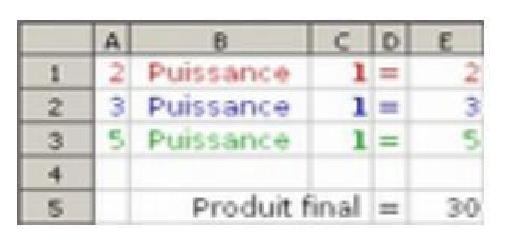
\includegraphics[width=.8\linewidth]{Pacti3}
\end{minipage}
\end{partie}
 \end{activite}
 
 
\begin{activite}[Écriture décimale d'une puissance de 10]
\begin{enumerate}
\item Donne l'écriture décimale des nombres suivants : $10^3$ ; $10^5$ et $10^9$.
\item Recopie puis complète : « L'écriture décimale de $10^{12}$ est un 1 suivi de ... zéros. »
\item Écris sous la forme d'une puissance de 10 les nombres suivants : 
	100 ; 1 000 000 et 1 000 000 000 000 000 000 000.
\item Donne l'écriture décimale des nombres suivants : $10^{-2}$ ; $10^{-6}$ et $10^{-8}$.
\item Recopie puis complète : « L'écriture décimale de $10^{-12}$ comporte ... zéros suivis d'un 1 (la virgule étant placée après le premier ...). »
\item À l'aide de la calculatrice, écris sous la forme d'une puissance de 10 les nombres suivants : 
 0,001 ; 0,000 000 01 et 0,000 000 000 000 000 1.
\end{enumerate}
\end{activite}


\begin{activite}[Toutes sortes de puissances]
\begin{partie}[Des chinois sous différentes formes]

La Chine compte actuellement environ 1 300 000 000 habitants. Donne le nombre d'habitants de la Chine en milliards. Combien cela fait-il en millions ? Et en milliers ?

Complète : $1 300 000 000 = ... \times 10^9 = ... \times 10^6 = ... \times 10^3$.
\end{partie}

\vspace{1em}
\begin{partie}[Distances astronomiques]

Dans le domaine de l'astronomie, le parsec sert à mesurer de très grandes distances entre les astres. Un parsec correspond à environ $3,086 \times 10^{16}$ m.

Complète : 1 parsec = $,086 \times 10^{16}$ m = ... cm = ... km = ... mm.
\end{partie}

\vspace{1em}
\begin{partie}[Globules rouges]

La taille moyenne d'un globule rouge est $7 \times 10^{-6}$ m.

Complète : $7 \times 10^{-6}$ m = ... cm = ... mm.
\end{partie}
\end{activite}

\begin{activite}[Opérations avec des puissances de 10]

\begin{partie}[Produit de puissances de 10]

\[ 10^2 \times 10^3 = \underbrace{\underbrace{10 \times 10}_{\text{... facteurs}} \times \underbrace{10 \times 10 \times 10}_{\text{... facteurs}}}_{\text{... facteurs au total}} = 10^{...}  \qquad \quad 10^5 \times 10^4 = \underbrace{\underbrace{10 \times ... \times 10}_{\text{... facteurs}} \times \underbrace{10 \times ... \times 10}_{\text{...facteurs}}}_{\text{... facteurs au total}} = 10^{...}  \]
      
\begin{enumerate}
\item Recopie puis complète les expressions ci-dessus.
\item Calcule de la même façon : $10^5 \times 10^8$ et $10^7 \times 10^6$.
\item Complète alors la formule suivante : 

Pour tous nombres entiers positifs $n$ et $p$ : $10^n \times 10^p = 10^{...}$.

\end{enumerate}
\end{partie}

\begin{partie}[Quotient de puissances de 10]
\begin{enumerate}
\item Si on décompose $\dfrac{10^5}{10^2}$, on obtient $\dfrac{10 \times 10 \times 10 \times 10 \times 10}{10 \times 10}$.

Simplifie cette fraction et donne le résultat sous la forme d'une puissance de 10.
\item Recommence avec les fractions suivantes : $\dfrac{10^7}{10^5}$ et $\dfrac{10^3}{10^2}$.
\item Complète alors la formule suivante :

Pour tous nombres entiers positifs $n$ et $p$ : $\dfrac{10^n}{10^p}=10^{...}$.
\end{enumerate}
\end{partie}

\begin{partie}[Puissance de puissances de 10]

\begin{enumerate}
\item Compte le nombre de facteurs 10 contenus dans l'écriture décomposée de $(10^2)^3$.
\item Recommence avec $(10^3)^5$. Combien aurait-on de facteurs 10 dans $(10^5)^8$ ?
\item Complète alors la formule suivante : 

Pour tous nombres entiers positifs $n$ et $p$ : $(10^n)^p=10^{...}$.
\end{enumerate}
\end{partie}
\end{activite}

